% $Id$

\chapter{Stochastic Search Programs}
\label{chapter:stochastic}

This section of \textsc{LALApps} contains programs that can be used to
search interferometer data for stochastic gravitational wave
backgrounds.

\clearpage
\section{Program \texttt{lalapps\_olapredfcn}}
\label{program:lalapps-olapredfcn}
\idx[Program]{lalapps\_olapredfcn}

\begin{entry}

\item[Name]
%
  \verb$lal_olapredfcn$ --- computes overlap reduction function given
  a pair of known detectors.

\item[Synopsis]
%
  \verb$lal_olapredfcn $[\verb$-h$]\verb$ $[\verb$-q$]\verb$ $[\verb$-v$]
  \verb$ $[\verb$-d debugLevel $]\verb+ \+\newline
  \verb$   $
  \verb$-s siteID1 $[\verb$-a azimuth1$]
  \verb$-t siteID2 $[\verb$-b azimuth2$]\verb+ \+\newline
  \verb$   $
  [\verb$-f fLow$]\verb$ -e deltaF$\verb$ -n numPoints$\verb$ -o outfile$
                         
\item[Description]
%
  \verb$lal_olapredfcn$ computes the overlap reduction function
  $\gamma(f)$ for a pair of known gravitational wave detectors.  It
  uses the LAL function \verb$LALOverlapReductionFunction()$, which is
  documented in the LAL Software Documentation under the
  \texttt{stochastic} package.

\item[Options]\leavevmode
\begin{entry}
\item[\texttt{-h}]
  Print a help message.
\item[\texttt{-q}]
  Run silently (redirect standard input and error to \texttt{/dev/null}).
\item[\texttt{-v}]
  Run in verbose mode.
\item[\texttt{-d} \textit{debugLevel}]
  Set the LAL debug level to \textit{debugLevel}.
\item[\texttt{-s} \textit{siteID1} \texttt{-t} \textit{siteID2}]
  Use detector sites identified by \textit{siteID1} and
  \textit{siteID2}; ID numbers between \texttt{LALNumCachedDetectors}
  (defined in the \texttt{tools} package of LAL) refer to detectors
  cached in the constant array \verb$lalCachedDetectors[]$.  (At this
  point, these are all interferometers.)  Additionally, the five
  resonant bar detectors of the IGEC collaboration can be specified.
  The bar geometry data (summarized in table~\ref{table:cachedBars})
  is used by the fucntion \verb$LALCreateDetector()$ from the
  \texttt{tools} package of LAL to generate the Cartesian position
  vector and response tensor which are used to calculate the overlap
  reduction function.  The ID numbers for the bars depend on the value
  of \texttt{LALNumCachedDetectors}; the correct ID numbers can be
  obtained by with the command
\begin{verbatim}
./lalapps_olapredfcn -h
\end{verbatim}
\item[\texttt{-a} \textit{azimuth1} \texttt{-b} \textit{azimuth2}]
%
  If \textit{siteID1} (\textit{siteID2}) is a bar detector, assume it
  has an azimuth of \textit{azimuth1} (\textit{azimuth2}) degrees East
  of North rather than the default IGEC orientation given in
  table~\ref{table:cachedBars}.  Note that this convention, measuring
  azimuth in degrees clockwise from North is not the same as that used
  in LAL (which comes from the frame spec).  Note also that any
  specified azimuth angle is ignored if the corresponding detector is
  an interferometer.
\item[\texttt{-f} \textit{fLow}]
  Begin the frequency series at a frequency of \textit{fLow}\,Hz; if this
  is omitted, the default value of 0\,Hz is used.
\item[\texttt{-e} \textit{deltaF}]
  Construct the frequency series with a frequency spacing of
  \textit{deltaF}\,Hz
\item[\texttt{-n} \textit{numPoints}]
  Construct a frequency series with \textit{numPoints} points.
\item[\texttt{-o} \textit{outfile}]
  Write the output to file \textit{outfile}.  The format of this file
  is that output by the routine \verb$LALPrintFrequencySeries()$ in
  the \texttt{support} package of LAL, which consists of a header
  describing metadata followed by two-column rows, each containing the
  doublet $\{f,\gamma(f)\}$.
\end{entry}

\begin{table}[tbp]
  \begin{center}
    \begin{tabular}{|c|c|c|c|}
\hline
      Name & Longitude & Latitude & Azimuth
\\ \hline
\verb$AURIGA$ & $11^\circ56'54''$E & $45^\circ21'12''$N & N$44^\circ$E 
\\ \hline
\verb$NAUTILUS$ & $12^\circ40'21''$E & $41^\circ49'26''$N & N$44^\circ$E 
\\ \hline
\verb$EXPLORER$ & $6^\circ12'$E & $46^\circ27'$N & N$39^\circ$E 
\\ \hline
\verb$ALLEGRO$ & $91^\circ10'43.\!\!''766$W & $30^\circ24'45.\!\!''110$N 
& N$40^\circ$W
\\ \hline
\verb$NIOBE$ & $115^\circ49'$E & $31^\circ56'$S & N$0^\circ$E 
\\ \hline
    \end{tabular}
    \caption{Location and orientation data for the five IGEC resonant
      bar detectors, stored in the \texttt{lalCachedBars[]}
      array.  The data are taken from
      \texttt{http://igec.lnl.infn.it/cgi-bin/browser.pl?Level=0,3,1}
      except for the latitude and longitude of ALLEGRO, which were
      taken from Finn \& Lazzarini, gr-qc/0104040.  Note that the
      elevation above the WGS-84 reference ellipsoid and altitude
      angle for each bar is not given, and therefore set to zero.}
    \label{table:cachedBars}
  \end{center}
\end{table}


\item[Example usage]
  To compute the overlap reduction function for LIGO Hanford and
  LIGO Livingston, with a resolution of 1\,Hz from 0\,Hz to 1024\,Hz:
\begin{verbatim}
lalapps_olapredfcn -s 0 -t 1 -e 1 -n 1025 -o LHOLLO.dat
\end{verbatim}
  
  To compute the overlap reduction function for ALLEGRO in its optimal
  orientation of $72.\!\!^\circ08$ West of South (see Finn \& Lazzarini,
  gr-qc/0104040) and LIGO Livingston, with a resolution of 0.5\,Hz from
  782.5\,Hz to 1032\,Hz (assuming \texttt{lalNumCachedBars} is 6):
\begin{verbatim}
lalapps_olapredfcn -s 9 -a 252.08 -t 1 -f 782.5 -e 0.5 -n 500 -o ALLEGROLHO.dat
\end{verbatim}

\item[Author]
John T.~Whelan

\end{entry}


\clearpage
\section{Program \prog{lalapps\_stochastic\_pipe}}
\label{program:lalapps-stochastic-pipe}
\idx[Program]{lalapps\_stochastic\_pipe}

\begin{entry}
\item[Name]
\prog{lalapps\_stochastic\_pipe} --- python script to generate Condor DAGs
to run the stochastic pipeline.

\item[Synopsis]
\begin{verbatim}
  -h, --help               display this message
  -v, --version            print version information and exit

  -d, --datafind           run LSCdataFind to create frame cache files
  -s, --stochastic         run lalapps_stochastic

  -P, --priority PRIO      run jobs with condor priority PRIO

  -f, --config-file FILE   use configuration file FILE
  -l, --log-path PATH      directory to write condor log file
\end{verbatim}

\item[Description] \prog{lalapps\_stochastic\_pipe} generates a Condor DAG
to run the stochastic search pipeline. The configuration should specify
the parameters needed to run the jobs and must be specified with the
\verb$--config-file$ option. A file containing science segments to
analysed should be specified in the \verb$[input]$ section of the
configuration file with a line such as

\begin{verbatim}
segments = S2H1L1v03_selectedsegs.txt
\end{verbatim}

This should contain four whitespace separated columns:

\begin{verbatim}
  segment_id    gps_start_time    gps_end_time    duration
\end{verbatim}

that define the science segments to be used. Lines starting with an
octothorpe are ignored.

\item[Example]
Generate a DAG to run a stochastic search on a pair of interferometers
specified in the configuration file. The generated DAG is then submitted
with \texttt{condor\_submit\_dag}

\begin{verbatim}
> lalapps_stochastic_pipe --log-path /home/ram/dag_logs \
     --datafind --stochastic --config-file stochastic_H1L1.ini
> condor_submit_dag stochastic_H1L1.dag
\end{verbatim}

\item[Author]
Adam Mercer
\end{entry}

\clearpage
\section{Program \prog{lalapps\_stochastic\_bayes}}
\label{program:lalapps-stochastic-bayes}
\idx[Program]{lalapps\_stochastic\_bayes}

\begin{entry}
\item[Name]
\prog{lalapps\_stochastic\_bayes} --- python script to generate Condor DAGs
to run the stochastic bayesian pipeline.

\item[Synopsis]
\begin{verbatim}
  -h, --help               display this message
  -v, --version            print version information and exit

  -d, --datafind           run LSCdataFind to create frame cache files
  -s, --stochastic         run lalapps_stochastic

  -P, --priority PRIO      run jobs with condor priority PRIO

  -f, --config-file FILE   use configuration file FILE
  -l, --log-path PATH      directory to write condor log file
\end{verbatim}

\item[Description] \prog{lalapps\_stochastic\_bayes} generates a Condor
DAG to run the stochastic search bayesian pipeline. The configuration
should specify the parameters needed to run the jobs and must be
specified with the \verb$--config-file$ option. A file containing
science segments to analysed should be specified in the \verb$[input]$
section of the configuration file with a line such as

\begin{verbatim}
segments = S2H1L1v03_selectedsegs.txt
\end{verbatim}

This should contain
four whitespace separated columns:

\begin{verbatim}
  segment_id    gps_start_time    gps_end_time    duration
\end{verbatim}

that define the science segments to be used. Lines starting with an
octothorpe are ignored.

\item[Example]
Generate a DAG to run a stochastic search on a pair of interferometers
specified in the configuration file. The generated DAG is then submitted
with \texttt{condor\_submit\_dag}

\begin{verbatim}
> lalapps_stochastic_bayes --log-path /home/ram/dag_logs \
    --datafind --stochastic --config-file stochastic_H1L1_bayes.ini
> condor_submit_dag stochastic_H1L1_bayes.dag
\end{verbatim}

\item[Author]
Adam Mercer
\end{entry}

\clearpage
\section{Program \prog{lalapps\_stochastic}}
\label{program:lalapps-stochastic}
\idx[Program]{lalapps\_stochastic}

\begin{entry}
\item[Name]
\prog{lalapps\_stochastic} --- standalone stochastic analysis code.

\item[Synopsis]
\prog{lalapps\_stochastic} \newline \hspace*{0.5in}
\option{--help} \newline \hspace*{0.5in}
\option{--version} \newline \hspace*{0.5in}
\option{--verbose} \newline \hspace*{0.5in}
\option{--debug-level} \parm{N} \newline \hspace*{0.5in}
\option{--gps-start-time} \parm{N} \newline \hspace*{0.5in}
\option{--gps-end-time} \parm{N} \newline \hspace*{0.5in}
\option{--interval-duration} \parm{N} \newline \hspace*{0.5in}
\option{--segment-duration} \parm{N} \newline \hspace*{0.5in}
\option{--sample-rate} \parm{N} \newline \hspace*{0.5in}
\option{--resample-rate} \parm{N} \newline \hspace*{0.5in}
\option{--f-min} \parm{N} \newline \hspace*{0.5in}
\option{--f-max} \parm{N} \newline \hspace*{0.5in}
\option{--ifo-one} \parm{IFO} \newline \hspace*{0.5in}
\option{--ifo-two} \parm{IFO} \newline \hspace*{0.5in}
\option{--channel-one} \parm{CHANNEL} \newline \hspace*{0.5in}
\option{--channel-two} \parm{CHANNEL} \newline \hspace*{0.5in}
\option{--frame-cache-one} \parm{FILE} \newline \hspace*{0.5in}
\option{--frame-cache-two} \parm{FILE} \newline \hspace*{0.5in}
\option{--calibration-cache-one} \parm{FILE} \newline \hspace*{0.5in}
\option{--calibration-cache-two} \parm{FILE} \newline \hspace*{0.5in}
\option{--calibration-offset} \parm{N} \newline \hspace*{0.5in}
\option{--apply-mask} \parm{N} \newline \hspace*{0.5in}
\option{--mask-bin} \parm{N} \newline \hspace*{0.5in}
\option{--overlap-hann} \newline \hspace*{0.5in}
\option{--hann-duration} \parm{N} \newline \hspace*{0.5in}
\option{--high-pass-filter} \newline \hspace*{0.5in}
\option{--hpf-frequency} \parm{N} \newline \hspace*{0.5in}
\option{--hpf-attenuation} \parm{N} \newline \hspace*{0.5in}
\option{--hpf-order} \parm{N} \newline \hspace*{0.5in}
\option{--recentre} \newline \hspace*{0.5in}
\option{--post-analysis} \newline \hspace*{0.5in}
\option{--middle-segment} \newline \hspace*{0.5in}
\option{--inject} \newline \hspace*{0.5in}
\option{--scale-factor} \parm{N} \newline \hspace*{0.5in}
\option{--seed} \parm{N} \newline \hspace*{0.5in}
\option{--trials} \parm{N} \newline \hspace*{0.5in}
\option{--output-dir} \parm{DIR} \newline \hspace*{0.5in}
\option{--test} \newline \hspace*{0.5in}
\option{--test-interval} \parm{N} \newline \hspace*{0.5in}
\option{--test-segment} \parm{N} \newline \hspace*{0.5in}
\option{--test-trial} \parm{N} \newline \hspace*{0.5in}
\option{--geo-hpf-frequency} \parm{N} \newline \hspace*{0.5in}
\option{--geo-hpf-attenuation} \parm{N} \newline \hspace*{0.5in}
\option{--geo-hpf-order} \parm{N}

\item[Description] \prog{lalapps\_stochastic} runs the standalone
stochastic analysis code.

\item[Options]\leavevmode
\begin{entry}
\item[\option{--help}]
Display usage information
\item[\option{--version}]
Display version information
\item[\option{--verbose}]
Run in verbose mode, code display set by set progress information
\item[\option{--debug-level} \parm{N}]
Sets the LAL Debug Level to \parm{N}
\item[\option{--gps-start-time} \parm{N}]
Sets the GPS time from which data should be read to \parm{N}
\item[\option{--gps-end-time} \parm{N}]
Sets the GPS time to which data should be read to \parm{N}
\item[\option{--interval-duration} \parm{N}]
Sets the interval duration to \parm{N}
\item[\option{--segment-duration} \parm{N}]
Sets the segment duration to \parm{N}
\item[\option{--sample-rate} \parm{N}]
Sets the sample rate of the input data to \parm{N}
\item[\option{--resample-rate} \parm{N}]
Sets the resample rate to \parm{N}
\item[\option{--f-min} \parm{N}]
Sets the minimum frequency of the search band to \parm{N}
\item[\option{--f-max} \parm{N}]
Sets the maximum frequency of the search band to \parm{N}
\item[\option{--ifo-one} \parm{IFO}]
Sets the IFO for the first stream to be \parm{IFO}, currently supported
IFO's are H1, H2, L1 and G1
\item[\option{--ifo-two} \parm{IFO}]
Sets the IFO for the second stream to be \parm{IFO}, currently supported
IFO's are H1, H2, L1 and G1
\item[\option{--channel-one} \parm{CHANNEL}]
Sets the channel for the first stream to be \parm{CHANNEL}
\item[\option{--channel-two} \parm{CHANNEL}]
Sets the channel for the second stream to be \parm{CHANNEL}
\item[\option{--frame-cache-one} \parm{FILE}]
Sets the frame cache file for the first stream to be \parm{FILE}
\item[\option{--frame-cache-two} \parm{FILE}]
Sets the frame cache file for the second stream to be \parm{FILE}
\item[\option{--calibration-cache-one} \parm{FILE}]
Sets the calibration cache file for the first stream to be \parm{FILE}
\item[\option{--calibration-cache-two} \parm{FILE}]
Sets the calibration cache file for the second stream to be \parm{FILE}
\item[\option{--calibration-offset} \parm{N}]
Sets the calibration offset to \parm{N}
\item[\option{--apply-mask}]
Apply frequency masking
\item[\option{--mask-bin} \parm{N}]
Set the number of bins to mask per frequency to \parm{N}
\item[\option{--overlap-hann}]
Use overlapping Hann windows for data segments
\item[\option{--hann-duration} \parm{N}]
Set the Hann duration of the data segment window to \parm{N}, 0 for
Rectangular windowing, 1 for Tukey windowing and 60 for Hann windowing
\item[\option{--high-pass-filter}]
Apply a high pass filter to the input data
\item[\option{--hpf-frequency} \parm{N}]
Set the knee frequency of the high pass filter to \parm{N}
\item[\option{--hpf-attenuation} \parm{N}]
Set the attenuation coefficent for the high pass filter to \parm{N}
\item[\option{--hpf-order} \parm{N}]
Sets the high pass filter order to \parm{N}
\item[\option{--recentre}]
Centre the data
\item[\option{--post-analysis}]
Perform post analysis
\item[\option{--middle-segment}]
Include the middle segment in the power spectra estimation
\item[\option{--inject}]
Perform signal injection
\item[\option{--scale-factor} \parm{N}]
Set the scale factor for injections to \parm{N}
\item[\option{--seed} \parm{N}]
Set the random seed for injections to \parm{N}
\item[\option{--trials} \parm{N}]
Set the number of trials for injections to \parm{N}
\item[\option{--output-dir} \parm{DIR}]
Set the output directory for search results to \parm{DIR}
\item[\option{--test}]
Save out intermediate products
\item[\option{--test-interval} \parm{N}]
Save out interval \parm{N}
\item[\option{--test-segment} \parm{N}]
Save out segment \parm{N}
\item[\option{--test-trial} \parm{N}]
Save out trial \parm{N}
\item[\option{--geo-hpf-frequency} \parm{N}]
Set the knee frequency for the GEO high pass filter to \parm{N}
\item[\option{--geo-hpf-attenuation} \parm{N}]
Set the attenuation coefficient for the GEO high pass filter to \parm{N}
\item[\option{--geo-hpf-order} \parm{N}]
Set the GEO high pass filter order to \parm{N}
\end{entry}

\item[Example]

\item[Author] 
Adam Mercer, Tania Regimbau
\end{entry}
\clearpage

\subsection{Pipeline Description}

\begin{figure}[htbp]
\begin{center}
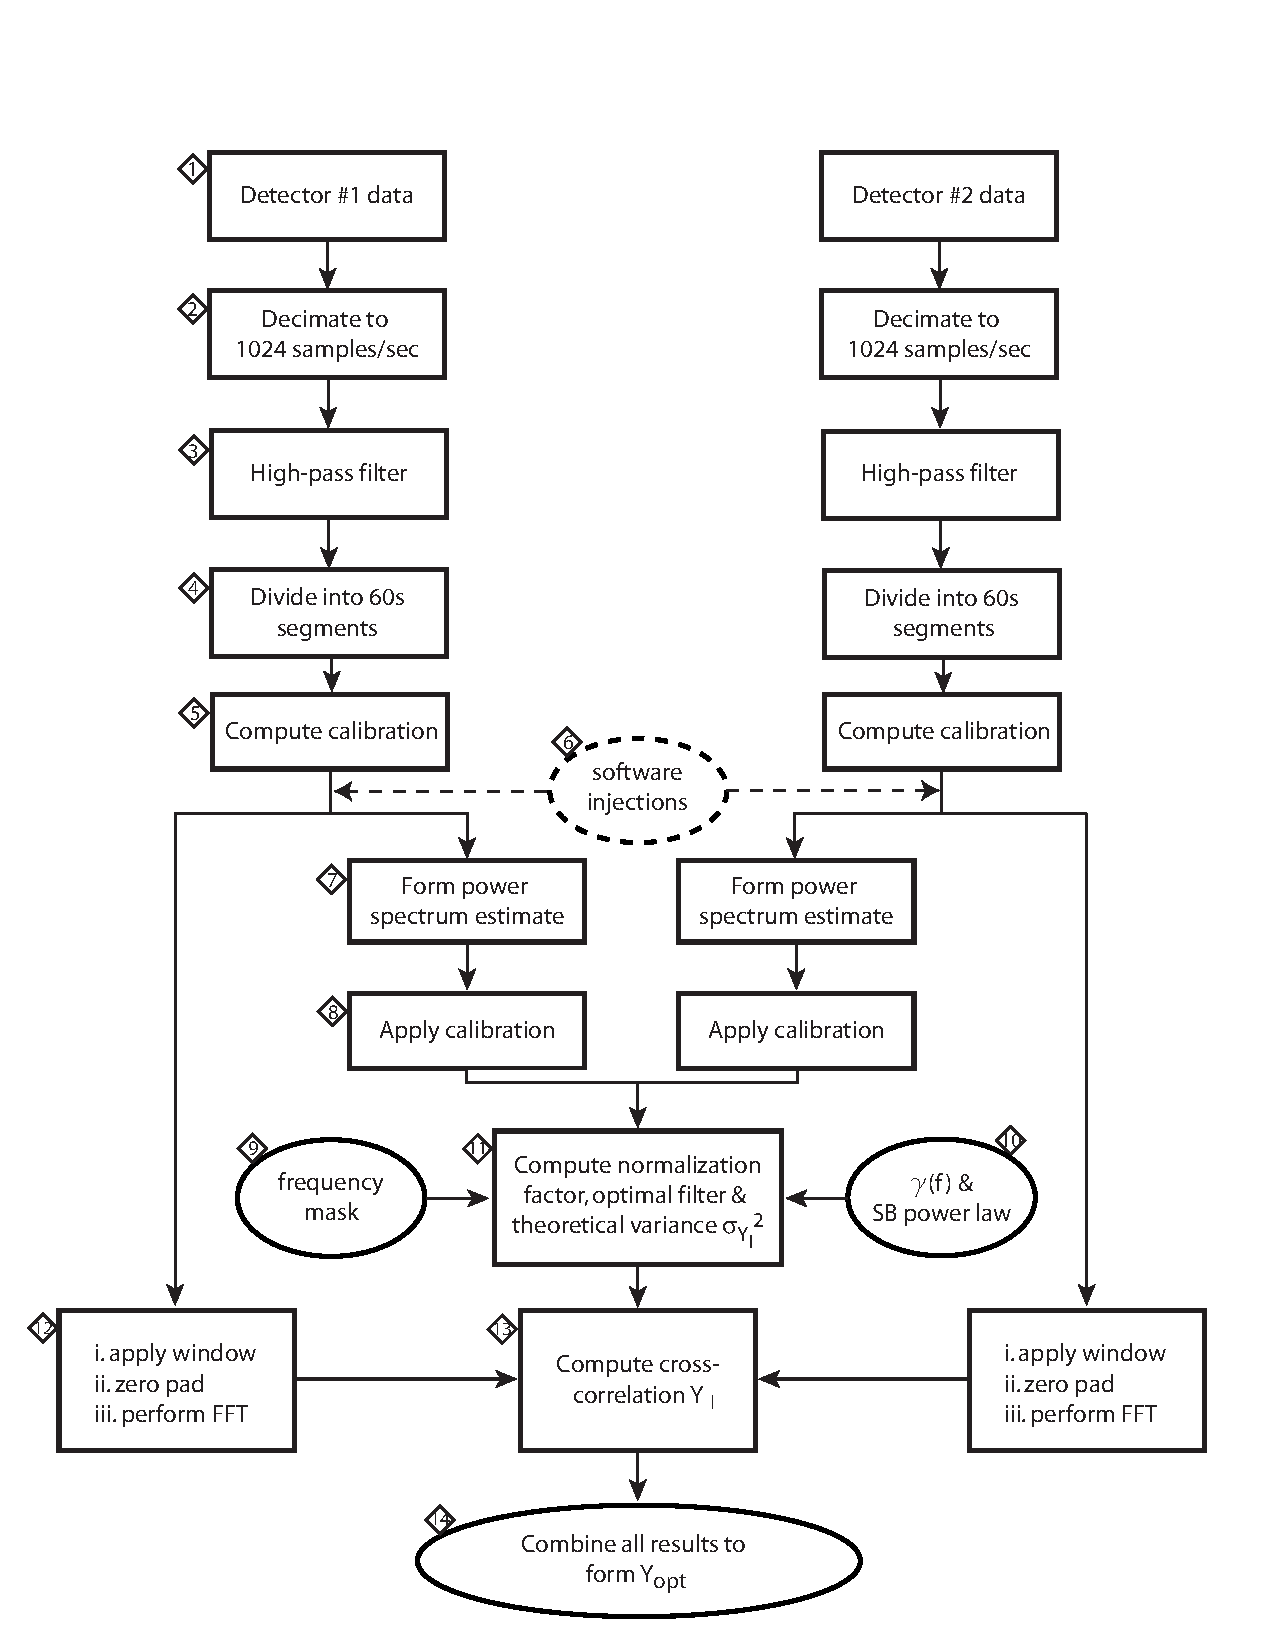
\includegraphics[width=5.5in]{figures/stochastic_flowdiagram.pdf}
\caption{Pipeline data flow diagram. Refer to the following text
	for descriptions of the blocks. The text is indexed by the numbers
  given in the diamonds next to the blocks.}
\label{fig:blockdigram}
\end{center}
\end{figure}

\begin{enumerate}

\item \textbf{Data selection:}
\begin{itemize}
\item We identify GPS start times and stop times of all double
coincident valid data using segwizard. For S2, all data quality flags
were set except MICHFILT (since MICHFILT removes a significant amount of
data which are useful for the stochastic analysis).
\item Using the segwizard GPS start and stop times, raw strain data
(Xn:LSC-AS\_Q) of length $\ge 62$~sec are read in from RDS-3 or raw
frames. 60 seconds is the minimum size data stretch that we analyze. The
extra 2 seconds is to account for filter transients introduced by
downsampling and high pass filtering (details below).
\end{itemize}

\item \textbf{Data decimation:}
Each data stretch pair is optionally high-pass filtered. For S2, we use
a 6th-order Butterworth filter with a knee frequency (-3 dB) of 40 Hz.
The first and last second of the downsampled, high-pass filtered data
stretches are discarded to avoid corruption from filter transients.

\item \textbf{Data partitioning:}
The downsampled, high-pass filtered data stretches are partitioned into
segments of length 60~sec. We choose 60~sec for the analysis of the S2
data to match the sample rate of the calibration data.

\item \textbf{Compute calibration:}
Transfer functions (units of counts/attostrain) for each IFO are
calculated from the frame-based calibration files for each 60-sec data
segment, using the calibration data whose GPS time lies within this
60-sec segment.

\item \textbf{Software injections:}
Simulated stochastic GW signals are injected into the data at this
stage, if desired. The simulated GW strain data are multiplied by the
instrument transfer functions in the frequency domain. This yields
simulated detector output (units of counts) for a stochastic
gravitational wave background which can be directly added to the raw
data.

\item \textbf{Power spectrum estimation:} 
Power spectra are estimated for each 60-sec data segment (including the
simulated stochastic GW signal, if it was injected into the data) using
Welch's method of averaged periodograms, with 50\% overlapping Hann
windows (4 second), and a 4-sec FFT length, corresponding to 29 averages
used in the estimate. The power spectra are used to construct the
optimal filter and theoretical variance for each of the 60-sec data
stretch pair. The units of the spectra are raw counts$^2$/Hz.

\item \textbf{Apply calibration:} 
The transfer functions are used to create two sets of calibrated power
spectra for each interferometer: fully calibrated power spectra (units
of strain$^2$/Hz) and half-calibrated power spectra (units of
strain$\cdot$count/Hz).

\item \textbf{Frequency mask:}
A frequency mask is created to remove discrete frequencies at which
instrumental correlations exist. The mask is simply a vector with zeros
at the positions corresponding to the discrete frequencies being
excised, and unity values everywhere else. For S2, the mask removes the
60 Hz mains frequency and its harmonics, as well as multiples of 16 Hz
(the GPS-synchronized data acquisition buffer rate). We remove a single
frequency bin (0.25 Hz bin width for S2) containing each of these lines.

\item \textbf{SB filter factors:}
\begin{itemize}
\item The overlap reduction function for the two sites is calculated.
\item The expected stochastic gravitational wave spectrum is set to
$\Omega_{\mathrm{gw}}(f)={\mathrm{const}}$.
\end{itemize}

\item \textbf{Normalization, optimal filter \& variance:}
\begin{itemize}
\item The normalization factor, $\cal N$ for the optimal filter and
theoretical variance, $\sigma_I$, for the CC statistic are calculated
using the overlap reduction function, fully calibrated power spectra,
and frequency mask. The summations over frequency to produce the
normalization and theoretical variance are restricted from
$f_{\mathrm{min}}$ to $f_{\mathrm{max}}$. For S2, we choose
$f_{\mathrm{min}} = 50$~Hz and $f_{\mathrm{max}}=300$~Hz. The lower
cutoff frequency is sufficiently greater than the knee frequency (40 Hz)
of the high-pass filter to avoid having to modify the response function
when calculating the optimal filter. The upper frequency yields more
than 95\% of the maximum obtainable SNR.
\item The optimal filter is constructed using the overlap reduction
function, normalization factor, frequency mask, and half-calibrated
power spectra. (The use of half-calibrated power spectra allows the
optimal filter to be applied directly to uncalibrated data when
calculating the cross-correlation spectrum.)
\end{itemize}

\item \textbf{Fourier transform:}
The 60-sec data segments are windowed, zero-padded to twice their length
(to avoid wrap-around problems when performing the correlation), and
discrete-Fourier-transformed (DFT) to the frequency domain. For S2, we
use either Tukey windows (with 0.5~s Hann turn-on and turn-off) or 50\%
overlapping Hann windows.

\item \textbf{Cross-correlation:}
\begin{itemize}
\item The cross-spectrum of the data pair is formed from the windowed,
zero-padded, and DFTed data segments, and this spectrum is
coarse-grained to match the frequency resolution and frequency cut-offs
of the optimal filter. The resultant frequency series is then
vector-multiplied with the optimal filter to yield the cross-correlation
spectrum (i.e., the integrand of the cross-correlation statistic).
\item The cross-correlation statistic value, $Y_I$, is calculated by
summing the cross-correlation spectrum values (from $f_{\mathrm{min}}$ to
$f_{\mathrm{max}}$), and multiplying by the frequency resolution (0.25~Hz).
\item The cross-correlation statistic value ($Y_I$) and theoretical
variance ($\sigma_I$) for each 60-sec data segment are written to a
file. A weighted sum of the cross-correlation spectra (using the inverse
theoretical variances) is also written to a file.
\end{itemize}

\item \textbf{Form $Y_{\mathrm{opt}}$:}
The cross-correlation statistic values for all 60-sec data segments are
optimally combined (weighting with the inverse variances), yielding a
single point estimate for $\Omega_0$ over the full data set. A single
statistical error bar on $\Omega_0$ is calculated from the theoretical
variances.

\end{enumerate}

\clearpage
\section{Program \prog{lalapps\_stopp}}
\label{program:lalapps-stopp}
\idx[Program]{lalapps\_stopp}

\begin{entry}
\item[Name]
\prog{lalapps\_stopp} --- Stochastic Post Processing.

\item[Synopsis]
\prog{lalapps\_stopp} \parm{options} \parm{xml files}\newline \hspace*{0.5in}
\option{--help} \newline \hspace*{0.5in}
\option{--version} \newline \hspace*{0.5in}
\option{--text} \newline \hspace*{0.5in}
\option{--output} \parm{FILE}

\item[Description] \prog{lalapps\_stopp} performs post processing upon
output from \prog{lalapps\_stochastic}.

\item[Options]\leavevmode
\begin{entry}
\item[\option{--help}]
Display usage information
\item[\option{--version}]
Display version information
\item[\option{--text}]
Output file as text
\item[\option{--output} \parm{FILE}]
write output data to \parm{FILE}
\end{entry}

\item[Example]

\item[Author]
Adam Mercer
\end{entry}
